% Option below is needed for minted
% !TEX options=--shell-escape

\documentclass{article}
\usepackage[T1]{fontenc}
% \usepackage{verbatim}

\usepackage{titlesec}
\usepackage{hyperref}

\usepackage[a4paper, margin=2.5cm, headsep=0pt]{geometry}

\usepackage{tgadventor}
\renewcommand{\familydefault}{\sfdefault}

\usepackage{graphicx}
\usepackage{titlepic}
\usepackage[skip=5pt]{caption}

\usepackage[ddmmyyyy]{datetime}
\usepackage[section]{placeins}
\usepackage{enumitem}

\usepackage[font=itshape]{quoting}

\titleformat{\chapter}{\normalfont\huge}{\bf\thechapter.}{20pt}{\huge\bf}
\titlespacing{\chapter}{0pt}{12pt plus 4pt minus 2pt}{8pt plus 2pt minus 2pt}

\hypersetup{
    colorlinks,
    citecolor=black,
    filecolor=black,
    linkcolor=black,
    urlcolor=blue
}

\newdate{creation}{22}{01}{2022}

\begin{document}
\begin{titlepage}
    \centering
    \vfill
    \bfseries\Huge{Pacenstein\\\large{- High Concept Document -}}\\
    \normalfont\normalsize\displaydate{creation}
    \vfill

    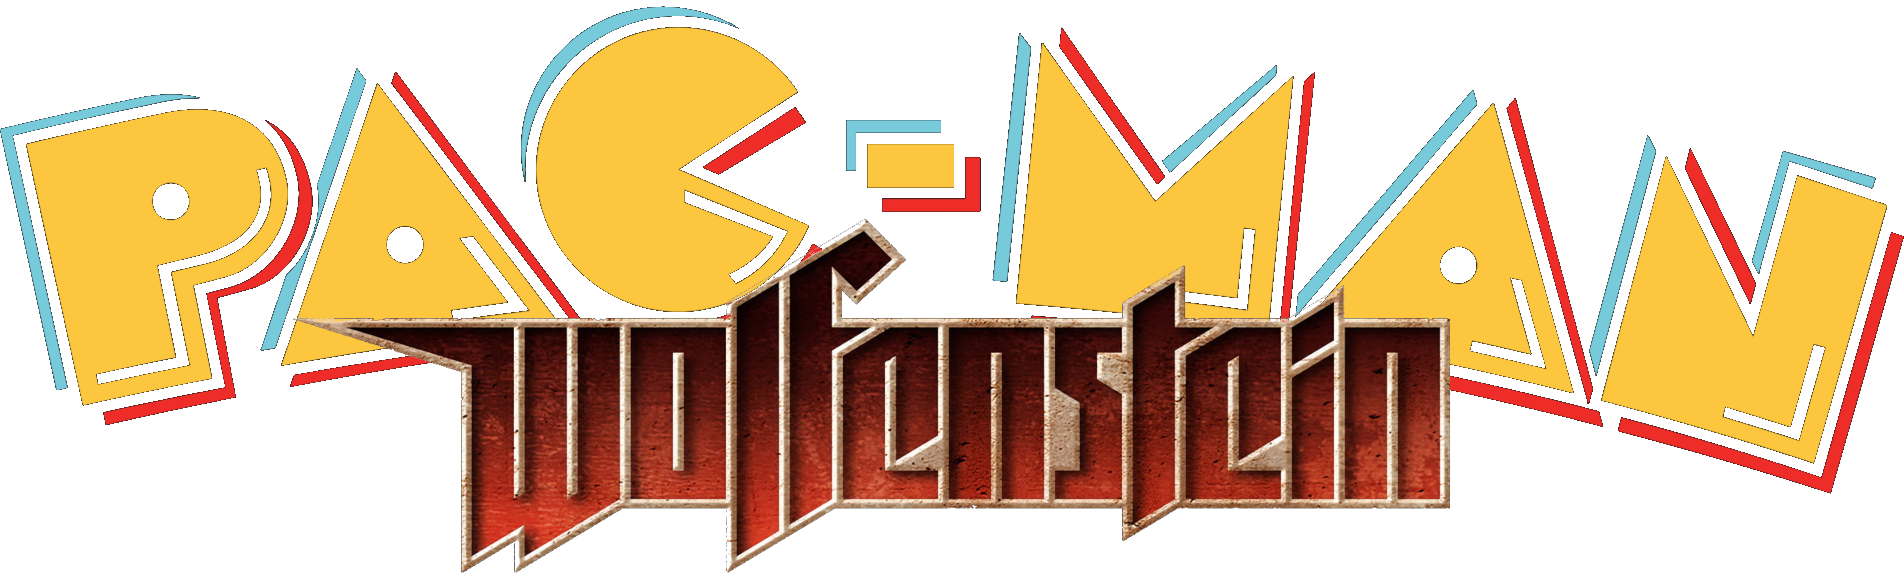
\includegraphics[width=\textwidth]{../res/pacenstein.png}
    \vfill
    \large{
        Lennard Duinkerken\\
        Emma Raijmakers\\
        Daan Roth\\
        Jarno Bröcker
    }
    \vfill
\end{titlepage}

% \maketitle
\newpage
\tableofcontents
\newpage

\section*{Inleiding} % (fold)
\label{sec:inleiding}
Tijdens dit gameproject wordt er een First Person Pacman game gerealiseerd door middel van raycasting. Deze game heeft de features van Pacman en het perspectief van Wolfenstein.
% section inleiding (end)

\section{Features \& Mechanics} % (fold)
\label{sec:features_&_mechanics}
\begin{itemize}[noitemsep]
    \item Je kan door een doolhof lopen.
    \item Overal in het doolhof zijn pac-dots - kleine bolletjes - geplaatst die punten opleveren.
    \item Je hebt drie levens.
    \item Je hebt de mogelijkheid bonuslevens te behalen als je een van de volgende scores hebt behaald:
    \begin{itemize}[noitemsep]
        \item Bij Easy difficulty is het elke 10.000 punten;
        \item Medium, 15.000;
        \item Hard, 20.000;
        \item En bij Impossible krijg je géén bonuspunten.
    \end{itemize}
    \item Er zijn 4 power-pellets - grote bolletjes - te vinden. Deze zorgen ervoor dat PacMan - de speler - de spoken kan opeten. Dan worden de spoken blauw en vluchten ze. Voor elk spook wat de speler opeet worden punten toebedeeld:
    \begin{itemize}[noitemsep]
        \item De eerste levert 200 punten op;
        \item De tweede 400;
        \item 800 voor de derde;
        \item En 1600 voor de laatste.
    \end{itemize}
    De spoken moeten wel achtereenvolgens opgegeten worden, na een aantal seconden stoppen de spoken met vluchten en jagen ze weer achter de speler aan.
    \item Als een spook is opgegeten dan gaat het naar het spookhuis. Daar komen ze weer tot ``leven''.
    \item De spoken knipperen wit om te laten weten dat ze bijna weer gevaarlijk worden.
    \item Zo nu en dan verschijnt er ``fruit'' dichtbij het midden. Het fruit levert bonuspunten op:
    \begin{itemize}[noitemsep]
        \item Cherry: 100 punten;
        \item Strawberry: 300;
        \item Orange: 500;
        \item Apple: 700;
        \item Melon: 1000.
    \end{itemize}
    \item De speler wordt achternagezeten door vier spoken, elk met een unike AI.
    \begin{itemize}[noitemsep]
        \item Het rode spook - Blinky - gaat rechtstreeks op PacMan af;
        \item Het cyaan spook - Inky - probeert PacMan tussen zichzelf en Blinky te krijgen;
        \item Het roze spook - Pinky - beweegt zich parallel aan PacMan in een poging hem te overvallen;
        \item Het oranje spook - Clyde - gaat rechtstreeks op PacMan af, maar wijkt af op het moment dat hij in de buurt komt.
    \end{itemize}
    \item De speler is in staat om PacMan te bedienen door middel van de W, A, S en D, of de pijltjestoetsen in te dukken.
    \item Het spel wordt 2.5D (3D-achtig, maar niet echt 3D) door een Raycasting engine te implementeren.
    \item De verschillende AI's voor de spoken maakt het spel spannender.
    \item Het spel heeft twee modi: Spoken jagen op, of ze vluchten voor PacMan.
    \item Aan het einde van het spel, wanneer de levens op zijn, kan de score opgeslagen en aan een leaderboard toegevoegd worden.
    \item \textbf{(Optioneel)} De muis kan gebruikt worden om links en rechts te kijken.
    \item \textbf{(Optioneel)} Achievements voor het behalen van een aantal punten, het eten van een aantal spoken, ...
    \item \textbf{(Optioneel)} Na levels twee, vijf en negen een korte cutscene invoegen, zogenaamd de ``Coffee break''. Dit zit ook in het originele spel: \href{https://pacman.fandom.com/wiki/Coffee_Break}{source}.
    \item Meer over de originele PacMan: \href{https://pacman.fandom.com/wiki/Pac-Man_(game)}{pacman.fandom.com/wiki}.
\end{itemize}
% section features_&_mechanics (end)

\section{Spelermotivatie} % (fold)
\label{sec:spelermotivatie}
Kort gezegd: hogere score = meer cool. Je score komt op een leaderboard waar je je naam aan toe kunt voegen, zo kunnen al je vrienden zien hoe hoog jouw score is. Daarna is het uiteraard de bedoeling dat ze de highscore neerzetten en deze zo lang mogelijk behouden.

Daarbij, PacMan is een alom bekend spel, en dit is niet anders dan de normale PacMan met een twist - de twist in dit geval is het 3D-effect.
% section spelermotivatie (end)

\section{Genre} % (fold)
\label{sec:genre}
First Person Maze Runner (?). Het is niet echt een genre wat een officiele naam heeft - naar mijn weten - maar first person maze runner is een aardige omschrijving van wat het inhoudt. Je kijkt vanuit het perspectief van het spelerskarakter - First Person - en beweegt door een doolhof - Maze Runner.
% section genre (end)

\section{Doelgroep} % (fold)
\label{sec:doelgroep}
Boomers.
\\\\
Haha grapje, maar ook weer niet eigenlijk. De baby boomer generatie is opgegroeid met PacMan en zal er een nostalgische waarde aan hechten en daarom dit spel willen spelen. Dit betekend niet dat het niet door andere mensen gespeeld kan/mag/wil worden, iedereen die PacMan kent en het in 3D wil ervaren valt onder onze doelgroep.
% section doelgroep (end)

\section{Competitie / Cooperatie} % (fold)
\label{sec:competitie_cooperatie}
Competitie vindt plaats via een leaderboard, jij wil de hoogste score en je vrienden ook... May the best player win.
\\\\
Cooperatie is niet van te spreken, het spel is puur ``single player''.
% section competitie_cooperatie (end)

\section{Unique Selling Points} % (fold)
\label{sec:unique_selling_points}
Het is een ongebruikelijke twist op een welbekende, klassieke game.
% section unique_selling_points (end)

\section{Doelplatform} % (fold)
\label{sec:doelplatform}
Er is specifiek op Intel $x86_64$ compatible hardware of, iets breder, PC's gericht.

Daarnaast kan onze game in princiepe op elk systeem draaien waar de GNU C-Compiler op beschikbaar is en waarop een bijpassende versie van SFML te includen valt. Ook is een toetsenbord en muis vereist, we implementeren niet expliciet de mogelijkheid om het spel met een touchscreen te bedienen. Maar als jij op je iPhone een compiler en SFML weet te krijgen, en vervolgens een toetsenbord en muis aan sluit - allereerst kudo's :p - dan staat het je vrij de source te downloaden, te compilen, en de game te spelen.
% section doelplatform (end)

\section{Ontwerpdoelen} % (fold)
\label{sec:ontwerpdoelen}
Het product is geslaagd op het moment er een PacMan game staat die voldoet aan minstens 90\% van de bovengenoemde criteria. Of alomvattend, als er een PacMan game staat die een 3D-achtige omgeving kan weergeven waar de speler doorheen kan lopen, op basis van Raycasting, met spoken erdoorheen bewegend.
% section ontwerpdoelen (end)

\section{Achtergrond} % (fold)
\label{sec:achtergrond}
\begin{quoting}
    Pac-Man, formerly known as Puck Man in Japan, is the main protagonist of the Pac-Man series. He is the husband of Ms. Pac-Man, and the father of Baby Pac-Man and Jr. Pac-Man.

    The Ghosts (also known as Monsters or Ghost Monsters) are the main enemies of the Pac-Man series and have antagonized Pac-Man and all of Pac-Land in their appearances. The most notable ghosts are the four members of the Ghost Gang - Blinky, Pinky, Inky and Clyde - who have appeared throughout the series as both antagonists and protagonists.
\end{quoting}
\small{Source: \url{https://pacman.fandom.com/wiki/Pac-Man_Wiki}}
\\\\
Pac-Man heeft de taak om zoveel mogelijk pac-dots opeten, de Monsters vinden dit niet leuk en proberen Pac-Man te stoppen.
% section achtergrond (end)
\end{document}
